Este filtro consiste en procesar una im\'agen para lograr un efecto miniatura. Consiste en que los objetos se vean pequeños o como de juguetes. Para esto se ''desenfoca'' la parte superior y la inferior de la im\'agen, quedando as\'i s\'olo el foco en la parte del medio, logrando tal efecto.



\subsubsection{Implementación en C}
Para esta implementaci\'on procesamos la imagen por bandas.
Para eso calculamos el límite de las bandas seg\'un los par\'ametros de entrada. Luego recorremos mediante dos ciclos la banda del medio y la dejamos igual, no hacemos ninguna transformaci\'on.\\
Luego dentro de un ciclo que cuenta las iteraciones, hacemos el procesamiento de ''desenfoque'' de la banda superior primero y luego la inferior.\\
Para desenfocar una banda, se recorre mediante dos ciclos que me permiten levantar cada color de cada pixel. Teniendo un componente de color de un pixel, se calcula el nuevo valor que debe tener el mismo. Para este c\'alculo se procesa la subimagen que hay alrededor del píxel, haciendo el c\'alculo por color, la multiplicamos por la matriz M, y vamos acumulando ese producto.\\
Para evitar la saturaci\'on, al resultado lo dividimos por 6, que es la suma de las componentes de la matriz M. Con el nuevo valor obtenido, lo pasamos a la im\'agen resultante. Seguimos procesando hasta finalizar la banda.
Para incrementar el efecto, lo que hacemos es, por iteraci\'on, guardar el p\'ixel desenfocado, para que en la siguiente iteración lo procese otra vez.\\

$M = \begin{pmatrix}
  0.01 & 0.05 & 0.18 & 0.05 & 0.01 \\
  0.05 & 0.32 & 0.64 & 0.32 & 0.05 \\
  0.18 & 0.64 & 1 & 0.64 & 0.18 \\
  0.05 & 0.32 & 0.64 & 0.32 & 0.05 \\
  0.01 & 0.05 & 0.18 & 0.05 & 0.01 \\
 \end{pmatrix}$

\subsubsection{Implementación en Assembler}
Para la implementaci\'on en assembler de este filtro, la diferencia mas sifnificativa contra la implementaci\'on en C, fue la forma de levantar los registros.
Usando los registros \emph{XMM} se levantaron 5 registros de 16 bytes cada uno de forma que al procesar la matriz se pudo reducir la cantidad de accesos a
 memoria y as\'i mejorar la performance. Se consideraron dos opciones a la hora de diseñar este filtro:\newline

\begin{itemize}
 \item Levantar de a 5 registros y avanzar bajando de a una fila y utilizando los 5 registros anteriores dejando 4 iguales y ahorrandome 4 accesos y pisando
el primer registro con la nueva fila de abajo. La imagen muestra la idea:
\begin{center}
 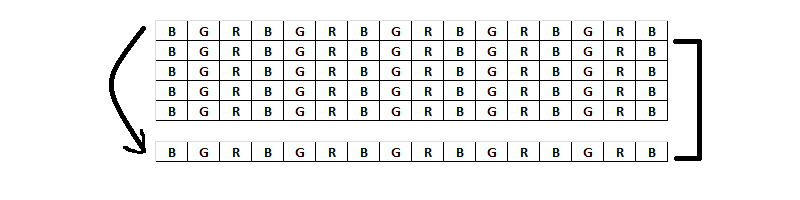
\includegraphics[scale=0.7]{imagenes/mover1.png}
\end{center}

\item El otro propuesto fue, levantar esos 5 registros pero en lugar de mover 1 registro hacia abajo, aprovechar la cache del procesador moviendonos hacia
la derecha ya que cuando copiamos de memoria un registro de 16 bytes traemos con el mucha mas informaci\'on que queda en cache con lo cual al movernos hacia
de esta manera estamos aprovechando los HIT de la cache en lugar de un MISS por cada iteraci\'on del ciclo. A continuaci\'on una imagen de lo propuesto.\newline
\begin{center}
 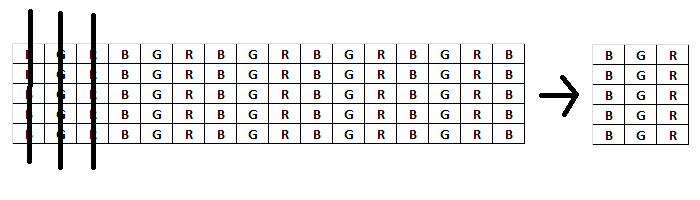
\includegraphics[scale=0.7]{imagenes/mover2.png}
\end{center}
Finalmente se opto por la segunda opci\'on por cuestiones de performance. El resto de las cuestiones estructurales como ciclos y operaciones son muy
similares al C.
\end{itemize}


\subsubsection{Resultados}
Comparando ambas implementaciones, notamos que estructuralmente no cambian mucho. En ambas tenemos la misma idea de ir recorriendo las bandas por un lado e ir haciendo la cuenta para el nuevo p\'ixel por otro. De todas formas, lo que se destaca es que en ASM tenemos menos accesos a memoria, ya que procesamos de a 5 p\'ixels, mientras que en C lo hacemos de a uno.\\
Adem\'as se puede apreciar que el ensamblado del compilador de C, al no usar SIMD se producen m\'as comparaciones que el ASM para terminar de recorrer la im\'agen.
En cuanto a la performance confirmamos lo que hab\'iamos supuesto, el ASM result\'o ser m\'as r\'apido que el C.\\

\begin{center}
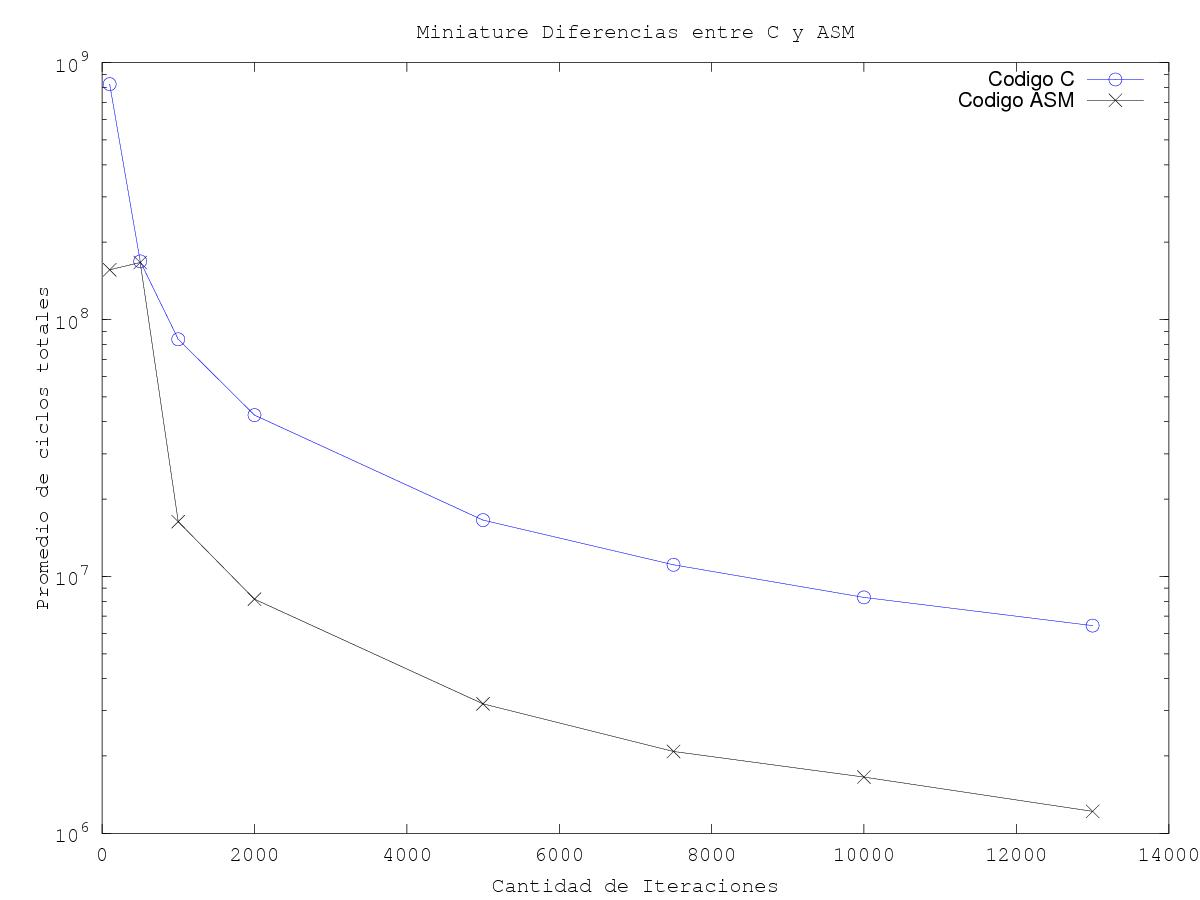
\includegraphics[width=16cm]{imagenes/medicionMiniature.jpg}  
\end{center}

Como podemos ver en el gr\'afico, lo que tarda la ejecuci\'on en promedio, el C se mantiene a la misma distancia del ASM a medida que aumentan las iteraciones, siempre tardando m\'as tiempo.\\

Experimentamos con varios tamaños de im\'agenes y pudimos ver que la diferencia en velocidad no cambia mucho. El C sigue tardando m\'as que el ASM, y con im\'agenes mas grandes hasta puede tardar m\'as que lo que vimos en el gr\'afico anterior.\\
Consideramos que a la hora de hacer este tipo de filtros, lo m\'as prioritario para optimizar es evitar los accesos a memoria lo m\'as posible, ya que como sabemos es una de las cosas m\'as costosas en cuanto a performance.\\



